% begin module e-definition
\begin{frame}
\[
\textrm{If } f(x) = a^x, \qquad f'(x) = f'(0)a^x .
\]
The simplest differential formula occurs when $f'(0) = 1$.  Since $\lim_{h\rightarrow 0}\frac{2^h-1}{h}\approx 0.69$ and $\lim_{h\rightarrow 0}\frac{3^h-1}{h}\approx 1.10$, we expect there is a number $a$ between 2 and 3 such that $\lim_{h\rightarrow 0}\frac{a^h-1}{h} = 1$.  
\uncover<2->{
\begin{definition}[$e$]
$e$ is the number such that $\lim_{h\rightarrow 0}\frac{e^h-1}{h} = 1$.
\end{definition}
}
\uncover<3->{%
\begin{columns}[c]
\column{.4\textwidth}
\ \only<handout:0| -6>{%
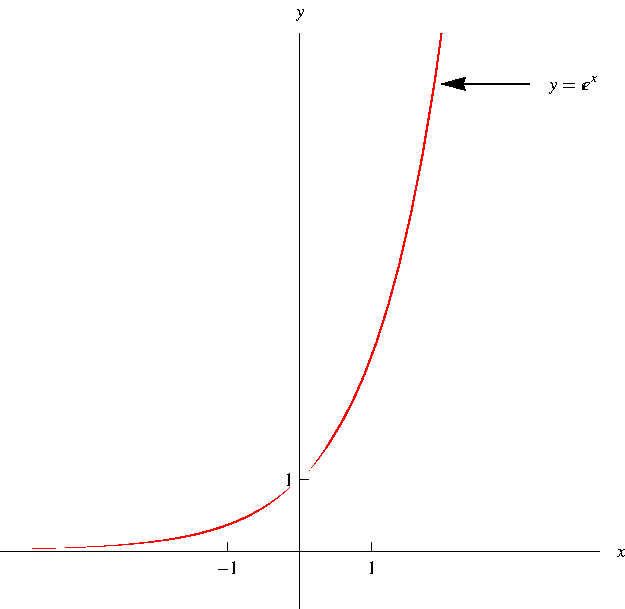
\includegraphics[height=4cm]{exponential-functions/pictures/07-02-natexpa.pdf}%
}%
\only<7->{%
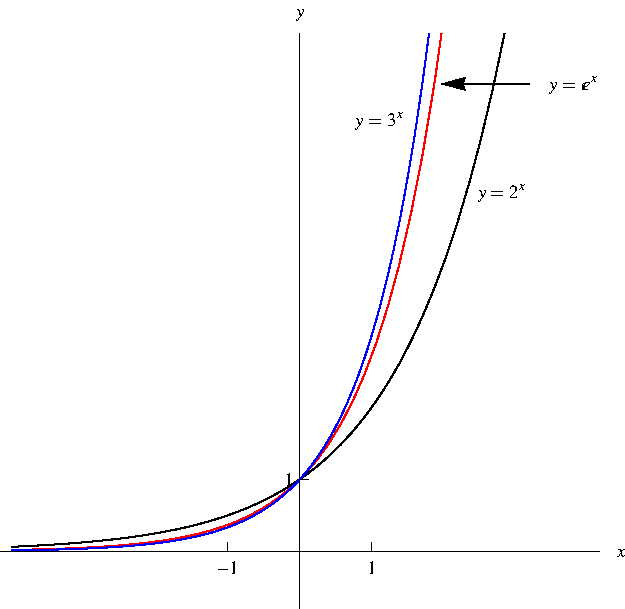
\includegraphics[height=4cm]{exponential-functions/pictures/07-02-natexpb.pdf}%
}%
\column{.6\textwidth}
\begin{itemize}
\item<3->  $f(x) = e^x$ has slope 1 at $x = 0$.
\item<4->  $\lim_{x\rightarrow \infty} e^x = \infty$.
\item<5->  $\lim_{x\rightarrow -\infty} e^x = 0$.
\item<6->  $e$ is a number between 2 and 3.
\item<7->  The graph of $y = e^x$ is between $y = 2^x$ and $y = 3^x$.
\end{itemize}
\end{columns}
}%
\end{frame}
% end module e-definition
